\documentclass[10pt,twoside,a4paper]{article}
% http://www-h.eng.cam.ac.uk/help/tpl/textprocessing/latex_maths+pix/node6.html symboles de math
% http://fr.wikibooks.org/wiki/Programmation_LaTeX Programmation latex (wikibook)
%=========================== En-Tete =================================
%--- Insertion de paquetages (optionnel) ---
\usepackage[french]{babel}   % pour dire que le texte est en fran{\'e}ais
\usepackage{a4}	             % pour la taille   
\usepackage[T1]{fontenc}     % pour les font postscript
\usepackage{epsfig}          % pour gerer les images
%\usepackage{psfig}
\usepackage{amsmath, amsthm} % tres bon mode mathematique
\usepackage{amsfonts,amssymb}% permet la definition des ensembles
\usepackage{float}           % pour le placement des figure
\usepackage{verbatim}

\usepackage{multicol} % multicolonnes

\usepackage{longtable} % pour les tableaux de plusieurs pages

\usepackage[table]{xcolor} % couleur de fond des cellules de tableaux

\usepackage{lastpage}

\usepackage{multirow}

\usepackage{multicol} % pour {\'e}crire dans certaines zones en colonnes : \begin{multicols}{nb colonnes}...\end{multicols} 

% \usepackage[top=1.5cm, bottom=1.5cm, left=1.5cm, right=1.5cm]{geometry}
% gauche, haut, droite, bas, entete, ente2txt, pied, txt2pied
\usepackage{vmargin}
\setmarginsrb{0.20cm}{0.20cm}{0.20cm}{0.20cm}{15pt}{3pt}{42pt}{15pt}

	
%\usepackage{frbib} % enlever pour obtenir references en anglais
% --- style de page (pour les en-tete) ---
\pagestyle{empty}

% mettre du texte en diagonale sur le fond : tikz
\usepackage{tikz} 
\def\confidentialTIKZ{%
	\begin{tikzpicture}[remember picture,overlay]
	\node[rotate=60,scale=15,text opacity=0.1] at (current page.center) {Confidentiel};
	\end{tikzpicture}
}%

\def\TIKZcyberpunkRED{%
	\begin{tikzpicture}[remember picture,overlay]
	\node[rotate=60,scale=10,text opacity=0.1] at (current page.center) {-- Cyberpunk RED};
	\end{tikzpicture}
}%

\usepackage{tikzpeople}

\def\txtTITLE{Feuille de personnage Cyberpunk RED} %%%%% !! TITRE !! %%%%%
\def\imgCORNER{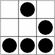
\includegraphics[width=0.25cm]{../../../../../images/glider/logo-glider.png}}

\def\imgGLIDERLEFTT{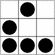
\includegraphics[width=1.95cm]{../../../../../images/glider/logo-glider-left.png}}
\def\imgGLIDERRIGHT{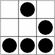
\includegraphics[width=1.95cm]{../../../../../images/glider/logo-glider-right.png}}

\def\imgGLIDERLEFTTsmall{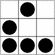
\includegraphics[width=0.25cm]{../../../../../images/glider/logo-glider-left.png}}
\def\imgGLIDERRIGHTsmall{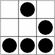
\includegraphics[width=0.25cm]{../../../../../images/glider/logo-glider-right.png}}

% % % en-tete et pieds de page configurables : fancyhdr.sty

% http://www.trustonme.net/didactels/250.html

% http://ww3.ac-poitiers.fr/math/tex/pratique/entete/entete.htm
% http://www.ctan.org/tex-archive/macros/latex/contrib/fancyhdr/fancyhdr.pdf
\usepackage{fancyhdr}
\pagestyle{fancy}
	% \renewcommand{\chaptermark}[1]{\markboth{#1}{}}
	% \renewcommand{\sectionmark}[1]{\markright{\thesection\ #1}}
\fancyhf{}
\fancyhead[LE,RO]{\bfseries\thepage \TIKZcyberpunkRED }
\fancyhead[LO]{\bfseries\rightmark}
\fancyhead[RE]{\bfseries\leftmark}
\fancyfoot[LE]{\thepage /\pageref{LastPage} \hfill
	\scriptsize{\txtTITLE} % TITLE
\hfill \imgGLIDERLEFTTsmall }
\fancyfoot[RO]{\imgGLIDERRIGHTsmall \hfill
	\scriptsize{\txtTITLE} % TITLE
\hfill \thepage /\pageref{LastPage}}
\renewcommand{\headrulewidth}{0.5pt}
\renewcommand{\footrulewidth}{0.5pt}
\addtolength{\headheight}{0.5pt}
% \fancypagestyle{plain}{
	% \fancyhead{}
	% \renewcommand{\headrulewidth}{0pt}
% }

\def\smallbox{%
	\setlength{\unitlength}{0.5cm}
	\fbox{
		\begin{picture}(1, 1)(0,0)
		\end{picture}
	}
}%

%%%%%%%%%%% SOME VALUES %%%%%%%%%%%%%%%%%%%%%
